\documentclass{book}
\usepackage{amssymb,amsmath}
\usepackage{polyglossia}
\setmainlanguage{spanish} % Idioma principal
\usepackage{theorem}
\usepackage{times}
\usepackage{array}
\usepackage{graphicx}
\usepackage{hyperref}
\usepackage{multirow}
\usepackage{fancyhdr}
%\usepackage[cp1252]{inputenc}
\usepackage{hhline}
\usepackage{multicol}
\usepackage[a4paper,driver=xetex,top=4.5cm,head=4.5cm, bottom=2cm,%
layouthoffset=0mm, left=2.5cm, right=2.5cm,marginparwidth=0cm]{geometry}
%\usepackage{bm}
%\usepackage{tabular}
\usepackage{fontspec}
 \usepackage[breakable,many]{tcolorbox}
\defaultfontfeatures{Ligatures=TeX}
\usepackage{empheq}
 \setromanfont{Roboto Condensed}
 \usepackage{float}
 \usepackage{mathrsfs} 
%
%
% \renewcommand{\familydefault}{\sfdefault}
%\renewcommand{\familydefault}{\sfdefault}

%%%%%%%%%Estilo de la pagina%%%%%%%%%%%%%%%%%%%%%%%%%%%%%%%%%%%
%%%%%%%%%%%%%%%%%%%%%%%%%%%%%%%%%%%%%%%%%%%%%%%%%%%%%%%%%%%%%%%%%%
% \newcounter{ejer}
% 
% {\theorembodyfont{\normalfont}
% \newtheorem{ejercicio}[ejer]{Ejercicio}}

\newcommand{\rr}{\mathbb{R}}
\newcommand{\qq}{\mathbb{Q}}
\newcommand{\nn}{\mathbb{N}}



\DeclareMathOperator{\atan2}{atan2}
%\DeclareMathOperator{\sen}{sen}
\DeclareMathOperator{\sign}{sign}
\DeclareMathOperator{\sn}{sn}
\DeclareMathOperator{\SO}{SO}
%\DeclareMathOperator{\arcsen}{arcsen}
\DeclareMathOperator{\Or}{O}

\usepackage[framemethod=TikZ]{mdframed}
%%%%%%%%%%%%%%%%%%%%%%%%%%%%%%
%Theorem

%% Ejercicio
\newcounter{ejer} \setcounter{ejer}{0}
\renewcommand{\theejer}{\arabic{ejer}}
\newenvironment{ejer}[2][]{%
\vspace{5pt}
\refstepcounter{ejer}%
\ifstrempty{#1}%
{%
% \mdfsetup{%
% frametitle={%
% \tikz[baseline=(current bounding box.east),outer sep=-0pt]
% \node[anchor=east,rectangle,fill=green!50]
{\noindent\bfseries Ejercicio~\theejer}.}
%
{%
% \mdfsetup{%
% frametitle={%
% \tikz[baseline=(current bounding box.east),outer sep=0pt]
% \node[anchor=east,rectangle,fill=green!50]
{\noindent\bfseries  Ejercicio~\theejer:~#1};}%
%
%\mdfsetup{innertopmargin=10pt,linecolor=green!50,%
%linewidth=2pt,topline=true,%
%frametitleaboveskip=\dimexpr-\ht\strutbox\relax
%}
%\begin{mdframed}[]
\relax%
\label{#2}}{\vspace{5pt}}%\end{mdframed}}

%Theorem
\newcounter{theo}[chapter] \setcounter{theo}{0}
\renewcommand{\thetheo}{\arabic{section}.\arabic{theo}}
\newenvironment{theo}[2][]{%
\refstepcounter{theo}%
\ifstrempty{#1}%
{\mdfsetup{%
frametitle={%
\tikz[baseline=(current bounding box.east),outer sep=0pt]
\node[anchor=east,rectangle,fill=blue!20]
{\strut Teorema~\thetheo};}}
}%
{\mdfsetup{%
frametitle={%
\tikz[baseline=(current bounding box.east),outer sep=0pt]
\node[anchor=east,rectangle,fill=blue!20]
{\strut Teorema~\thetheo:~#1};}}%
}%
\mdfsetup{innertopmargin=10pt,linecolor=blue!20,%
linewidth=2pt,topline=true,%
frametitleaboveskip=\dimexpr-\ht\strutbox\relax
}
\begin{mdframed}[]\relax%
\label{#2}}{\end{mdframed}}
%%%%%%%%%%%%%%%%%%%%%%%%%%%%%%
%Lemma
\newcounter{lem}[chapter] \setcounter{lem}{0}
\renewcommand{\thelem}{\arabic{section}.\arabic{lem}}
\newenvironment{lem}[2][]{%
\refstepcounter{lem}%
\ifstrempty{#1}%
{\mdfsetup{%
frametitle={%
\tikz[baseline=(current bounding box.east),outer sep=0pt]
\node[anchor=east,rectangle,fill=green!20]
{\strut Lemma~\thelem};}}
}%
{\mdfsetup{%
frametitle={%
\tikz[baseline=(current bounding box.east),outer sep=0pt]
\node[anchor=east,rectangle,fill=green!20]
{\strut Lemma~\thelem:~#1};}}%
}%
\mdfsetup{innertopmargin=10pt,linecolor=green!20,%
linewidth=2pt,topline=true,%
frametitleaboveskip=\dimexpr-\ht\strutbox\relax
}
\begin{mdframed}[]\relax%
\label{#2}}{\end{mdframed}}
%%%%%%%%%%%%%%%%%%%%%%%%%%%%%%
%% Definicion
\newcounter{defini}[chapter] \setcounter{defini}{1}
\renewcommand{\thedefini}{\arabic{section}.\arabic{defini}}
\newenvironment{definicion}[2][]{%
\refstepcounter{defini}%
\ifstrempty{#1}%
{\mdfsetup{%
frametitle={%
\tikz[baseline=(current bounding box.east),outer sep=0pt]
\node[anchor=east,rectangle,fill=green!20]
{\strut Definición~\thedefini};}}
}%
{\mdfsetup{%
frametitle={%
\tikz[baseline=(current bounding box.east),outer sep=0pt]
\node[anchor=east,rectangle,fill=green!20]
{\strut Definición~\thedefini:~#1};}}%
}%
\mdfsetup{innertopmargin=10pt,linecolor=green!20,%
linewidth=2pt,topline=true,%
frametitleaboveskip=\dimexpr-\ht\strutbox\relax
}
\begin{mdframed}[]\relax%
\label{#2}}{\end{mdframed}}

%Proof
\newenvironment{prf}{\noindent\emph{Dem.}}{$\square$ \newline\vspace{5pt}}


%Corolario
\newcounter{cor}[chapter] \setcounter{cor}{0}
\renewcommand{\thecor}{\arabic{section}.\arabic{cor}}
\newenvironment{cor}[2][]{%
\refstepcounter{cor}%
\ifstrempty{#1}%
{\mdfsetup{%
frametitle={%
\tikz[baseline=(current bounding box.east),outer sep=0pt]
\node[anchor=east,rectangle,fill=green!20]
{\strut Corolario~\thelem};}}
}%
{\mdfsetup{%
frametitle={%
\tikz[baseline=(current bounding box.east),outer sep=0pt]
\node[anchor=east,rectangle,fill=green!20]
{\strut Corolario~\thelem:~#1};}}%
}%
\mdfsetup{innertopmargin=10pt,linecolor=green!20,%
linewidth=2pt,topline=true,%
frametitleaboveskip=\dimexpr-\ht\strutbox\relax
}
\begin{mdframed}[]\relax%
\label{#2}}{\end{mdframed}}

\tcbset{highlight math style={enhanced,
  colframe=red!60!black,colback=yellow!50!white,arc=4pt,boxrule=1pt,
  drop fuzzy shadow}}
  
  
  
  
  
  
  


\pagestyle{fancyplain}

 \renewcommand{\sectionmark}[1]
                 {\markright{\thesection\ #1}}


% \lhead[\fancyplain{}{\bfseries\thepage}]
%       {\fancyplain{}{\bfseries\rightmark}}
%
 \rhead[\fancyplain{}{\bfseries\leftmark}]{\fancyplain{}{\bfseries}}




 \lhead[\fancyplain{}{ 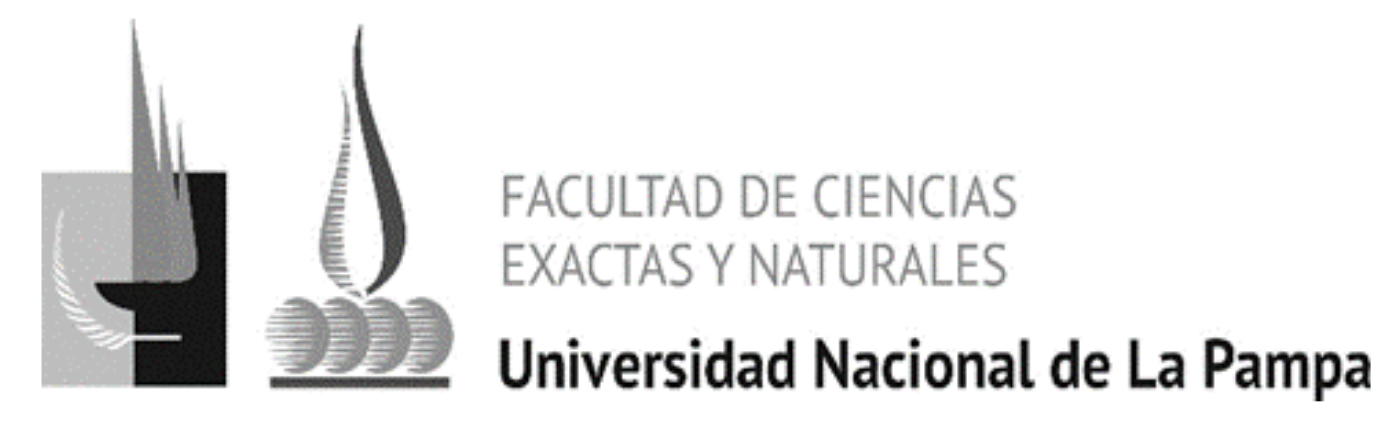
\includegraphics[scale=.3]{EscudoUNLPam.png}}]{\fancyplain{}{ 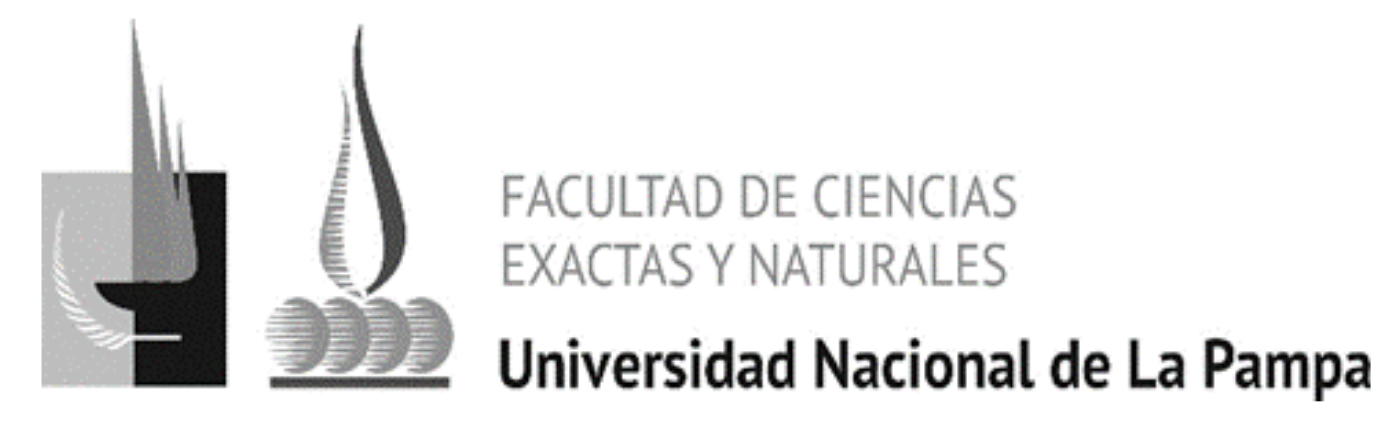
\includegraphics[scale=.3]{EscudoUNLPam.png}}}

\cfoot{}





  
  
  
  
  
  
  
\begin{document}


\hyphenation{excen-tri-ci-dad}


\begin{large}
\begin{bfseries} % \begin{scshape}
        \noindent Depto de Matem\'atica.\\
        Primer Cuatrimestre de 2022\\                                                                                                                                                                                                                                                                                                                                                
        Teoría de la Medida \\
        Práctica 7: Medidas abstractas

%\end{scshape}
\end{bfseries}
\end{large}
\par\noindent\rule{\textwidth}{.5pt}



\begin{ejer}{} Demostrar que los siguientes ejemplos definen álgebras de conjuntos.
 \begin{enumerate}
  \item La colección de todas las uniones de una cantidad finita de intervalos de $\mathbb{R}$, donde por intervalo entendemos tanto acotados como  no y tanto abiertos como cerrados o ninguno de ambos.
  \item Como en el ejemplo anterior, pero con los extremos de los intervalos en $\mathbb{Z}\cup \{\pm \infty\}$ ó $\mathbb{Q}\cup \{\pm \infty\}$.
    \item Más generalmente aún, como en los ejemplos anteriores, pero con los extremos de los intervalos en $A\cup \{\pm \infty\}$, donde $A\subset\mathbb{R}$.
 \end{enumerate}
\end{ejer}


\begin{ejer}{} Demostrar que los siguientes ejemplos definen clases monótonas.
 \begin{enumerate}
  \item La colección de todos los intervalos de $\mathbb{R}$ de la forma $(a,+\infty)$ ó $[a,+\infty)$ con $a\in [-\infty,+\infty)$.
  \item En $\mathbb{R}^n$ la colección de de todas las bolas, tanto cerradas como abiertas, de centro $0$ y radio $r\in[0,+\infty]$. 
  \item La colección de todos los subgrupos de un grupo dado $G$. 
 \end{enumerate}
\end{ejer}


\begin{ejer}{}
 Mostrar que  $\Sigma$ es $\sigma$-álgebra si y sólo si $\Sigma$ es álgebra y clase monótona.
\end{ejer}


\begin{ejer}{} Supongamos que $\mathscr{A}$ es un álgebra que  satisface  $\bigcup\limits_{n=1}^{\infty} E_n\in \mathscr{A},$
si $E_n \in \mathscr{A}$ para $ n=1,2,\ldots$ y  mutuamente disjuntos. Probar que $\mathscr{A}$ es $\sigma$-álgebra.
 
\end{ejer}
	
 

\begin{ejer}{}
 Verificar que $\mathscr{A}=\{(a,+\infty)|a \in \rr\}\cup \{[a,+\infty)|a \in \rr\}$ es clase mónotona pero no 
es álgebra.
\end{ejer}


\begin{ejer}[Medida de conteo]{def:med_cont} Sea $X$  un conjunto y $\mathscr{A}=\mathcal{P}(X)$ la colección de todos los subconjuntos de $X$. Para $A\in\mathscr{A}$, escribamos $\mu(A)=\#A$ cuando $A$ es finito, y $\mu(A)=+\infty$ cuando $A$ no es finito. Demostrar que el triple $(X,\mathscr{A},\mu)$ es espacio de medida.
 
\end{ejer}
 
 
\begin{ejer}{def:med_cont} Sea $X=\mathbb{N}$  y $\mathscr{A}=\mathcal{P}(\mathbb{N})$ la colección de todos los subconjuntos de $\mathbb{N}$. Supongamos que dada una función $f:\mathbb{N}\to [0,+\infty]$, para $A\in\mathscr{A}$ escribimos 
\[\mu(A)=\sum_{n\in A}f(n), \] 
Demostrar que el triple $(\mathbb{N},\mathscr{A},\mu)$ es espacio de medida. ¿Qué resulta $\mu$ si $f(n)=1$ para todo $n$? ¿Qué condición debe satisfacer $f$ para que $\mu(A)<\infty$ para todo $A\subset\mathbb{N}$?
 
\end{ejer}

\begin{ejer}{}  Sea $(X,\mathscr{A},\mu)$ espacio de medida. Demostrar que se satisfacen las siguientes relaciones
\begin{enumerate}
 \item $\mu(\emptyset)=0$.
 \item $\mu(A\cup B)+\mu(A\cap B)=\mu(A)+\mu(B)$.
 \item Si $\mu(B)<\infty$ y $B\subset A$ entonces $\mu(A-B)=\mu(A)-\mu(B)$. 
\end{enumerate}
\end{ejer}


\begin{ejer}{def:med_cont_mult3} Sean $X=\mathbb{N}$  y $\mathscr{A}=\mathcal{P}(\mathbb{N})$ la colección de todos los subconjuntos de $\mathbb{N}$. Sea $k$ un natural fijo. Para $A\subset\mathbb{N}$ escribimos
\[
 \mu(A)=\#\{ n\in A :  k|n \},
\]
es decir $\mu(A)$ cuenta cuántos múltiplos de $k$ hay en $A$. Demostrar que: 
\begin{enumerate}
    \item $\mu$ es medida;
    \item $\mu$ es una instancia de las medidas introducidas en \eqref {def:med_cont}. 
\end{enumerate}
\end{ejer}


\begin{ejer}[Delta de dirac]{ejer:delta_dirac}
 Sea $X$ un conjunto no vacío cualquiera, $a\in X$ un punto fijo y $\mathscr{A}=\mathcal{P}(X)$. Definimos $\delta_a:\mathscr{A}\to [0,+\infty]$ por
 \[
  \delta_a(A)=\left\{\begin{array}{ll} 1 &\text{ si } a\in A\\0 &\text{ si } a\notin A.\end{array}\right.
 \]
 Demostrar que $(X,\mathscr{A},\delta)$ es un espacio de medida. La medida $\delta_a$
se denomina \emph{$\delta$ de Dirac}. 
\end{ejer}
 

\begin{ejer}{} 
 Sea $\mu_0$ una premedida sobre el álgebra  $\mathscr{A}_0$ de subconjuntos de $X$. Definimos  $\mu^\star:\mathcal{P}(X)\to [0,+\infty]$ por
 \begin{equation}\label{eq:defi_med_ext}
  \mu^\star(E)=\inf\left\{ \sum_{j=1}^{\infty}\mu_0(E_j)\mid E\subset \bigcup_{j=1}^{\infty}E_j, E_j\in\mathcal{A}_0  \right\}
 \end{equation}
Probar que  $\mu^\star$ es una medida exterior. 

  
\end{ejer}

\begin{ejer}{} Demostrar que si $\mu$ es una medida sobre una $\sigma$-álgebra,  entonces $\mu(\emptyset)=0$.
\end{ejer}

\begin{ejer}{}
Sean $\mu^*$ medida exterior en $X$ y $\mathscr{A}$ el conjunto de todos los conjuntos  medibles Carathéodory.
Probar que:
\begin{enumerate}
\item $\emptyset  \in \mathscr{A}$;
\item si $\mu^{*}(E)=0$ entonces $E \in \mathscr{A}$.
\end{enumerate}
\end{ejer}

\begin{ejer}{} Supongamos que $g:\rr\to\rr$ es no decreciente y diferenciable con $g'$ continua. Sea $\mu_g$ la medida de Lebesgue-Stieltjes que genera $g$. Demostrar que para todo Boreliano $A\subset\rr$
\[
 \mu_g(A)=\int_Ag'(t)dt.
\]
\end{ejer}

\begin{ejer}{} Sea 
$$g(x)=\left\{
            \begin{array}{cl}
             -1  & \hbox{ si } x<0\\
             x  & \hbox{ si } 0\leq x < 1\\
             x^2  &   \hbox{ si } 1\leq x 
            \end{array}
       \right.
$$
y sea $\mu_g$ la medida de Lebesgue-Stieltjes que genera $g$. Calcular 
$\mu_g([-1,2])$
\end{ejer}



\end{document}
